

Antes de comenzar con el análisis descriptivo de nuestra base de datos es importante determinar si no existen datos datos faltantes, NA´s, en ella. Asegurando, de esta manera, que lo observado e interpretado de nuestros datos es correcto y no se presentan distorsiones por este problema. 
\\\\
De manera sencilla, con ayuda del software R y en particular con la función ``anyNA()`` observamos que nuestra base de datos esta completa y por ende continuamos con su análisis.
\\\\
En general, contamos con 4,581 precios al cierre registrados, como bien lo mencionábamos, comenzando el 23 de mayo de 2002 y terminando el 3 de agosto de 2020.

\begin{figure}[!ht]
    \centering
    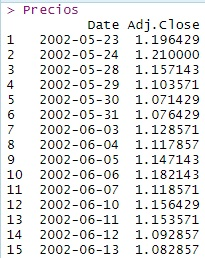
\includegraphics[scale=.75]{Graficos/HeadPrecios.jpg}
   \caption{Datos Log Rendimientos.}
    \label{Datos Log Rendimientos.}
\end{figure}

Algunas de las estadísticas más relevantes son las siguientes: El precio mínimo de cierre registrado fue de 0.37 dólares el 9 de octubre de 2002, mientras que el precio máximo de cierre se registró el 10 de julio de 2020 por un monto de 439.17 dólares. Por otro lado, Netflix presentó un promedio de precios al cierre por 72.82 dólares por acción a lo largo de estos 18 años y mostró una mediana de 14.54 dólares. 
\\\\
Asimismo, con ayuda de los cuantiles, observamos un sesgo a la izquierda, es decir, una simetría positiva que indica, en general, que el precio de cierre de Netflix se mantuvo en constante crecimiento.
\\\\
Finalmente corroboramos, a través del comando class(), que este dataset es del tipo series de tiempo y además su frecuencia o periodicidad es igual a 251.
\newpage
\subsection{Análisis Gráfico.}
A continuación mostramos las gráficas más representativas de nuestra base de datos, e interpretamos una a una, con el fin de tener un mayor conocimientos de nuestros datos antes de intentar ajustar algún modelo.
\begin{figure}[!ht]
    \centering
    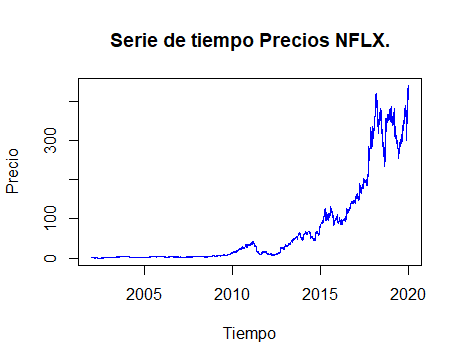
\includegraphics[scale=.75]{Graficos/PreciosNFLT.png}
   \caption{Precios Netflix.}
    \label{Precios Netflix.}
\end{figure}
\\\\

La gráfica anterior muestra los precios de cierre de Netflix, en la cual podemos observar, como bien se mencionaba en la ``Introducción a la Base``, que dichos precios se han visto afectados por diversos sucesos. En particular, se observa que: A partir de 2010 y hasta 2011, comienzan a subir los precios como respuesta al quiebre de Blockbuster y su apertura en América Latina y el Caribe; De manera similar, también se presenta una subida en 2015 a consecuencia de los 17 millones de nuevos usuarios. Finalmente, en 2019 muestra una importante caída como respuesta a una gran disminución en el número de usuarios y fallo de proyecciones de ventas a nivel mundial.   

Por otro lado, se observa en general una varianza creciente, por lo cual proseguiremos a transformar los datos, obteniendo como resultado el siguiente gráfico.

\begin{figure}[!ht]
    \centering
    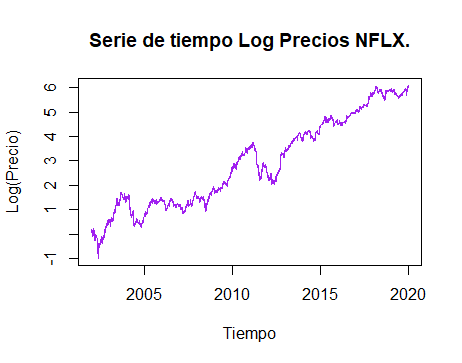
\includegraphics[scale=.70]{Graficos/LOGPRECIOSNFLT.png}
  \caption{Log Precios Netflix.}
    \label{Log Precios Netflix.}
\end{figure}
\newpage
A través de la figura \ref{Log Precios Netflix.} verificamos que nuestra transformación, la cual fue aplicar el logaritmo natural a los precios, resultó correcta, por el hecho de que se muestran un poco más compactos y con menos fluctuaciones.
\\\\
Posteriormente, de acuerdo con la teoría investigada, definimos una nueva transformación como la diferencia entre los precios logarítmicos, la cual nos permitirá trabajar de manera más adecuada, y al resultado lo llamaremos "Log Rendimientos". Como se muestra en la figura \ref{Log Rendimientos.}.

\begin{figure}[!ht]
    \centering
    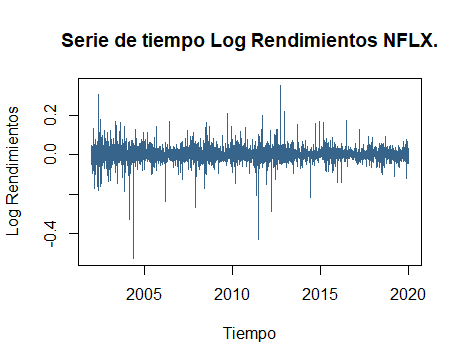
\includegraphics[scale=.7]{Graficos/Rendimientos.png}
  \caption{Log Rendimientos.}
    \label{Log Rendimientos.}
\end{figure}

Este gráfico será analizado con mayor detenimiento en secciones posteriores, pero a grandes rasgos vemos: no tendencia, oscilación alrededor del cero y la variabilidad va cambiando. Además de que muestra dos significativas caídas una antes de 2005 y otra en 2010. Junto con una gran subida entre 2010 y 2015.  
\\\\
\\\\
A continuación se muestran los histogramas de los Precios y los Log Precios de Netflix, con sus respectivas densidades empíricas. 

\begin{figure}[htbp]
    \centering
    \subfigure{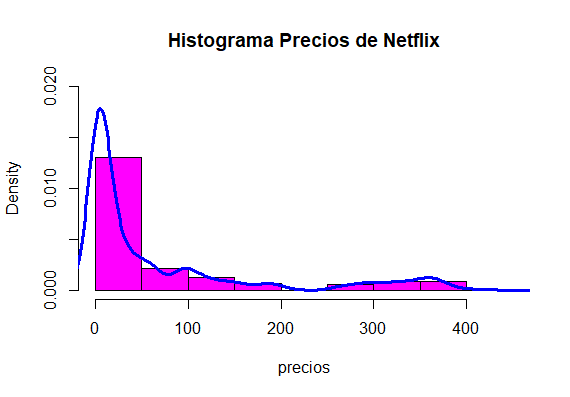
\includegraphics[width=60mm]{Graficos/HIstPreciosNFLX.png}}\vspace{10mm}
    \subfigure{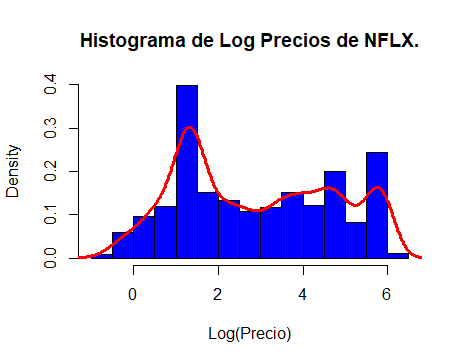
\includegraphics[width=60mm]{Graficos/Hist Log Precios NFLX.png}}
    \caption{Histogramas.} 
    \label{HistogramasPN.}
\end{figure}

Con lo que respecta al gráfico del lado izquierdo, notamos que la mayoría de los datos se concentran entre los 0 y 50 dólares, por lo cual podemos interpretar a los precios que oscilan más allá de los 400 dólares como valores atípicos dentro de nuestra serie de tiempo.
\\\\
Análogamente, el gráfico del lado derecho confirma nuestra interpretación, pues como bien sabemos, el aplicar una transformación logaritmo resulta en un reescalamiento de los datos. Por lo cual, seguimos notando un pico importante entre el 0 y el 2 del Log(Precio). 
\\\\
\newpage
Por último, presentamos el histograma correspondiente con los Log Rendimientos, así como su función de densidad empírica.
\\\\
\begin{figure}[htbp]
    \centering
    \subfigure{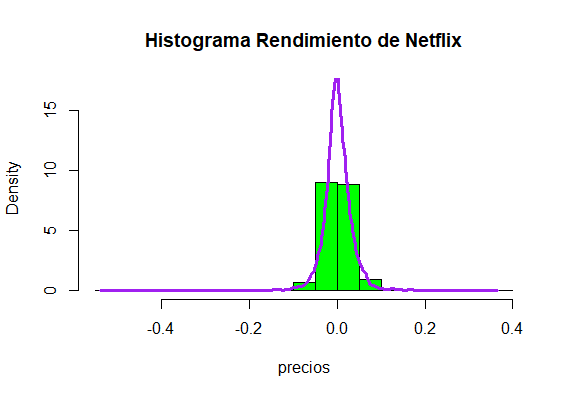
\includegraphics[width=80mm] {Graficos/Hist Log Rendi NFLX.png}}\vspace{10mm}
    \subfigure{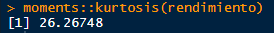
\includegraphics[width=55mm]{Graficos/Kurtosis.png}}
    \caption{Histograma Log Rendimientos} 
    \label{Histogramas Log Rendimientos.}
\end{figure}
\\\\
\\\\
Observemos que en general, se presentan colas muy pesadas, al igual que una kurtosis muy por encima de la que presentaría una distribución normal, estás características nos ayudarán a definir nuestro modelo más adelante.    




